\documentclass[12pt]{article}
\usepackage{amsmath,amssymb,amsthm}
\usepackage{graphicx,mathabx}
\usepackage{xcolor}
\usepackage{tikz}
\usepackage{cases}
\usepackage{placeins}
\usepackage{lipsum}
\usepackage{multirow}
\usepackage{mathtools}
\usepackage[shortlabels]{enumitem}
\usepackage{wrapfig}
\DeclarePairedDelimiter{\floor}{\lfloor}{\rfloor}
\begin{document}
\title{TCSS 343 - Week 3 - Monday}
\author{Jake McKenzie}
\maketitle
\noindent\centerline{\textbf{Stating Problems Formally and Master Method}}\\\\\\\\\\\\\\\\
\begin{center}
    ``The purpose of a storyteller is not to tell you how to think, but to give you questions to think upon." \\$\cdots$\\ Brandon Sanderson
\end{center}
\begin{center}
    ``Writing is nature's way of letting you know how sloppy your thinking is." \\
    $\dots$\\
    Guindon
\end{center}
\begin{center}
    ``Master method will never be sufficient for the detailed 'knuthian' analysis of algorithms, but they can free algorithm designers from mundane analyses to let them work on more interesting problems." \\$\cdots$\\ Jon Bentley, Dorothea Blostein et al (creators of the master method)  
\end{center}
\newpage
\noindent For this problem consider the algorithm ``drawCantorCircles'', on a specified canvas (square painting surface), 
draws a nested circle pattern, where the largest circle is centered a $(x,y)$ with a given radius and filled with colour1. 
There are two nested subpatterns, each with half the radius, internally tangent along the main horizontal diameter, with colours 
alternating between colour2 and colour1. No circle whose radius is less than a minimum radius is drawn.
\\
\centerline{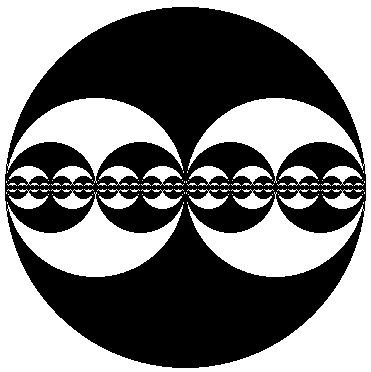
\includegraphics[scale = 2]{contor_circle.jpg}}
\begin{enumerate}
\item[0.]  Express this problem formally with input and output conditions.
\newpage
\item Describe a simple brute force algorithm to compute this picture assuming that it takes 
some constant amount of work to place each circle. How many circles does this algorithm draw asymptotically in 
the worst case?
\newpage
\item Assume that the radius of the first circle is greater than zero and divisible by $2$.
What type of picture will this algorithm output? Draw the picture.\\\\\\\\\\\\\\\\\\\\\\\\\\\\\\\\
\item Assume that the radius of the first circle is greater than zero and is \textbf{NOT} divisible by $2$.
What type of picture will this algorithm output? Draw the picture.
\newpage 
\item State a self-reduction for your problem.\\\\\\\\\\\\\\\\\\\\\\\\\\\\\\\\
\item State a recursive algorithm that solves the problem.
\newpage
\item State a tight asymptotic bound on the act of drawing a circle used by your algorithm in the worst case.
(HINT: develop a recurrence relation for your algorithm then use the Master Theorem to solve it)
\newpage
\item In this problem use the Master Theorem to find and prove tight bounds for the following recurrence.
\[
T(n) = \left\{
\begin{tabular}{cc}
c & \text{if} $n\leq 1$ \\
$9T\left(\left\lfloor\frac{n}{3}\right\rfloor\right)+3$ & \text{if} $n>1$ \\
\end{tabular}\right.
\]
\newpage
\item In this problem use the Master Theorem to find and prove tight bounds for the following recurrence.
\[
T(n) = \left\{
\begin{tabular}{cc}
c & \text{if} $n\leq 1$ \\
$3T\left(\left\lfloor\frac{n}{9}\right\rfloor\right)+3n$ & \text{if} $n>1$ \\
\end{tabular}\right.
\]
\newpage
\item In this problem use the Master Theorem to find and prove tight bounds for the following recurrence.
\[
T(n) = \left\{
\begin{tabular}{cc}
c & \text{if} $n\leq 1$ \\
$3T\left(\left\lfloor\frac{n}{2}\right\rfloor\right)+3n$ & \text{if} $n>1$ \\
\end{tabular}\right.
\]
\end{enumerate} 
\newpage
\end{document} 